% !Mode:: "TeX:UTF-8"
\chapter{分支预测针对解耦前端的设计}

本章首先介绍前端解耦的含义,以及为什么需要对前端解耦,之后详细介绍解耦前端的设计中分支预测相关部分的设计,主要是介绍FTQ (Fetch Target Queue) 的功能和设计,FTQ作为连接分支预测部件和取指部件的关键部件,在承担保存取指请求功能的同时也承担了保存分支预测信息和管理后端指令提交信息的功能,通过FTQ能够让以Fetch Block为基本单位的分支预测部件和以单条分支为基本单位的后端流水线进行信息的交互,以实现必要的功能。

\section{香山第一版耦合前端简介}

% 还没有介绍BPU的三级覆盖预测和分支历史管理机制
% 还没有介绍IUM
% 也没有讲各个部件SRAM尺寸的改变

在香山第一版的设计中,而我们把分支预测和取指统称为流水线的前端。相对的以译码为边界,译码和译码之后的流水级我们统称为后端。而在第一版的前端设计里,取指单元和分支预测的流水级是耦合在一起的,如图\ref{fig:figure41}所示。也就是说只有当分支预测和取指单元当前流水级都完成之后,才能够流向下一流水级,这会导致分支预测和指令缓存的访问互相阻塞。例如当访问指令缓存发现miss时,即使分支预测已经完成,也仍然需要停下来等待指令缓存从下级缓存中得到回填的数据;同样的当分支预测需要覆盖预测,冲刷流水线时,即使指令缓存已经准备好被访问了,由于流水线被冲刷,暂时没有新的访问请求,也只能够等待分支预测执行。这种相互掣肘的耦合关系通过解耦,可以将大量的前端气泡消除,即将分支预测流水线和取指流水线分离,中间由一个队列连接,这个队列就是FTQ (Fetch Target Queue)。

\begin{figure}[htb]
	\centering
	\setlength\tabcolsep{3pt}  % 同一行中的图片间隔
	\vspace{5pt} % 图片上部的空白,如果太小的话,图片顶部会与正文内容十分接近
	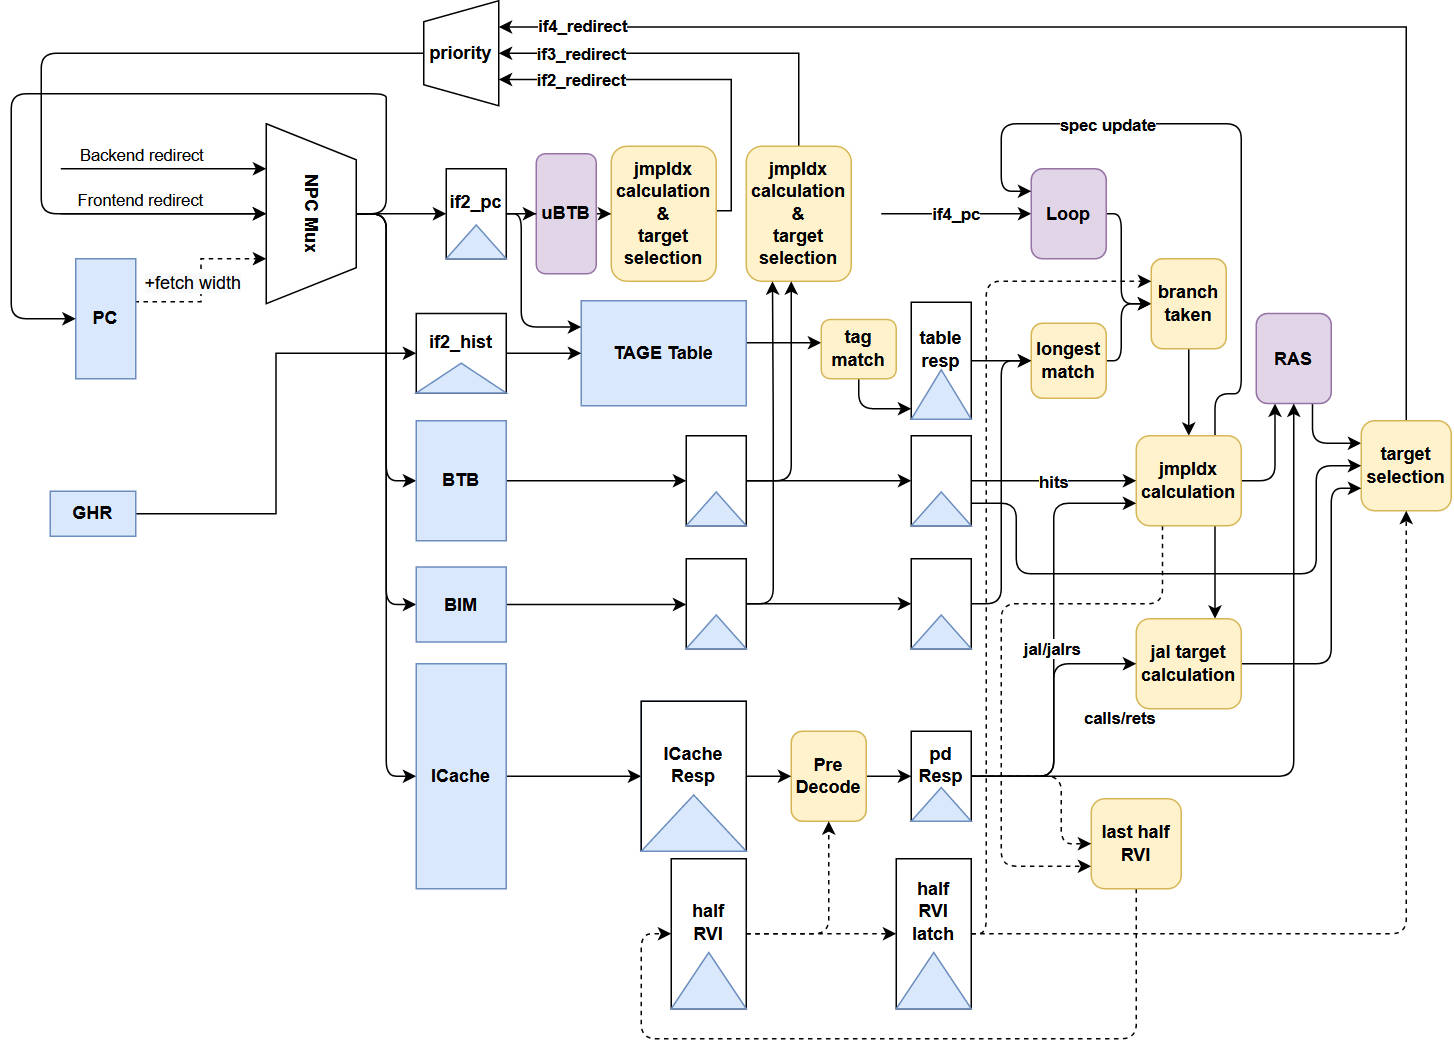
\includegraphics[width=1\textwidth]{yqh-IFU-BPU.jpg}
	\caption{香山处理器第一版分支预测与取指架构图}
    \label{fig:figure41}
\end{figure}

\section{通过FTQ实现前端解耦}

通过将分支预测流水线和取指流水线解耦开,通过FTQ连接,如图\ref{fig:figure21}所示,就能够将分支预测和取指单元变成类似于生产者和消费者的关系:分支预测作为生产者,负责不断地预测当前pc下一拍的取指pc,而不用管指令缓存是否miss,只需要将相关的取指请求放入FTQ之中。而取指单元作为消费者,负责不断地从FTQ中顺序取出取指的请求,访问指令缓存得到指令码,将它传给后端。由于在指令缓存miss时,分支预测仍旧会不断地往FTQ中送入取指请求,因此当分支预测冲刷流水线时,取指单元也不用等待,可以继续取出FTQ中之前存储的取指请求,继续访问指令缓存取指。这样一来就能够减少前端很多不必要的气泡,前端的供指效率能够得到提高,这也会对整体架构的性能有一定的正面影响。

FTQ属于连接分支预测部件、取指部件和后端的一个连接组件。

FTQ中使用的指针由flag和value两个属性。这种数据结构在香山的其他部件中也有应用。

由于FTB在指令提交更新时有时需要先花一个周期去读FTB,因此FTQ需要控制在这种时候不能够连续发2次指令提交信号给分支预测

FTQ对列中有四个指针,分别代表当前流水线中指令执行的不同进度:

\begin{enumerate}
	\item bpuPtr
	\item ifuPtr
	\item ifuwbPtr
	\item commPtr
\end{enumerate}

FTQ中有效的项在bpuPtr和commPtr之间

FTQ会接收BPU s2和s3的信号,当分支预测部分有redirect时,FTQ中也要将指针恢复到正确的位置

每次有取指请求入队时,FTQ需要给分支预测返回新入队的项的bpuPtr,在分支预测redirect时需要用这个指针进行恢复。

取指请求在分支预测S1 fire和S2,S3 redirect的时候发送给FTQ

FTQ中的存储结构(或者说FTQ表项中的组成部分)主要有:

\begin{itemize}
	\item ftq\_pc\_mem。在分支预测有新的取指请求,以及分支预测redirect时写入,主要修改取指请求中的pc和其他相关属性
	\item ftq\_redirect\_sram。用于保存分支预测redirect时需要的一些信息,例如RAS栈顶元素和栈顶指针,全局历史指针等。在分支预测最后一个流水级fire时写入
	\item ftq\_meta\_1r\_sram。用于保存所有预测器在预测时产生的meta信息,是一个很长的UInt,将所有的meta信息都转成UInt拼接起来,拼接和拆分由Composer组件负责。在分支预测最后一个流水级fire时写入
	\item ftb\_entry\_mem。存放分支预测传来的FTB表项。在分支预测最后一个流水级fire时写入
	\item ftq\_pd\_mem。用来存储预译码信息
\end{itemize}

update\_target
cfiIndex\_vec
mispredict\_vec
pred\_stage

commitStateQueue。用来表示每个FTQ项代表的Fetch Block中所有指令的状态,分别有invalid,valid,commited三个状态

entry\_fetch\_status。用来表示FTQ项对应的取指状态

entry\_hit\_status。用来表示FTQ项在FTB的hit状态,有not\_hit,hit和false\_hit。

当分支预测s2和s3需要redirect时,FTQ要负责把bpuPtr和ifuPtr都移动到正确的位置。同时把redirect信号发给IFU,IFU对之前的错误的取指进行恢复

FTQ有bypass操作,如果上一拍BPUfire,且ifuPtr等于当前的bpuPtr,就直接将最新的取指请求发给IFU

FTQ还要接收从IFU写回的信息,在取指请求发给IFU,IFU取回指令码,并预译码之后,会将预译码信息传回FTQ保存起来,同时IFU还会检测是否有明显的误预测,如果有也会发给FTQ,由FTQ给分支预测发送误预测恢复信号。并将commitStateQueue有效的指令状态修改为valid

写回后还会和之前保存的FTB entry进行判断,有没有false\_hit,当FTB hit,但是预译码结果和FTB entry中的结果不一致时,则认为是出现了false\_hit的情况,具体可能有是分支不是分支,是跳转不是跳转,以及跳转目标地址的offset不同

FTQ还要将指令信息传给后端,由后端执行时再做一次判断,决定是否误预测

当后端发现误预测指令时,后端回发回误预测信号和误预测指令所在block的FtqPtr,FTQ根据这个指针去读取ftq\_redirect\_sram和ftb\_entry\_mem中的数据,将这些数据进行处理后发送回分支预测,并更新分支历史

IFU发的redirect也和后端的处理方式类似

RedirectGen。接收后端发来的信息,生成redirect信号

恢复指针和state queue。在有误预测时,需要恢复FTQ的指针和状态队列,redirect的来源有后端和IFU,同时发redirect时以后端的优先,在redirect发生时,无论是后端还是IFU,都会发回发生redirect的block在FTQ中对应的指针,我们需要将bpuPtr,ifuPtr,ifuwbPtr都恢复到redirect 指针加1的位置,因为误预测的指令所在的block也是需要提交的。同时需要将block中误预测指令之后的所有指令的状态都置为invalid。

后端发redirect时,FTQ不光要给分支预测发redirect,也要给IFU发

每当有指令提交时,FTQ需要将对应指令的状态修改为commited

当一个block中的所有指令状态是invalid或commited,并且其中有跳转的指令,或者曾在FTB中命中,那么block就可以向分支预测提交了。提交时我们会把ftq\_pc\_mem,ftq\_pd\_mem,ftq\_redirect\_sram,ftq\_meta\_1r\_sram,ftb\_entry\_mem中commPtr中对应的数据都取出来,用于生成传给分支预测的分支预测训练数据。

FTQ会控制发送commit的频率,如果某次更新FTB需要先查找FTB再写入,那么FTQ就会将之后的commit请求延后,等到FTB准备好下一次更新时再发送。

FTB中表项的更新逻辑由FtbEntryGen中实现

FTQ还有一些支持指令预取的逻辑

\section{分支历史管理策略}

\section{本章小结}

